\documentclass[tikz,border=7pt]{standalone}
\usepackage{iftex}
\ifPDFTeX
  \PackageError{matrix-figure}{This figure requires XeTeX or Tectonic}{Compile with xelatex or tectonic.}
\fi
\usepackage{fontspec}
\usepackage{xeCJK}
\usepackage{amsmath}
\usepackage{unicode-math}
\usepackage{xcolor}
\usepackage{tikz}
\usetikzlibrary{arrows.meta,positioning}

\providecommand{\FigureUseLocalFonts}{0}
\ifnum\FigureUseLocalFonts=1
  \setmainfont{NotoSansCJKtc-Regular.otf}[Path=\FigureSansFontPath]
  \setsansfont{NotoSansCJKtc-Regular.otf}[Path=\FigureSansFontPath,BoldFont=NotoSansCJKtc-Bold.otf]
  \setCJKmainfont{NotoSansCJKtc-Regular.otf}[Path=\FigureSansFontPath]
  \setCJKsansfont{NotoSansCJKtc-Regular.otf}[Path=\FigureSansFontPath,BoldFont=NotoSansCJKtc-Bold.otf]
  \setmathfont{STIXTwoMath.otf}[Path=\FigureMathFontPath]
\else
  \setmainfont{Noto Sans CJK TC}
  \setsansfont{Noto Sans CJK TC}
  \setCJKmainfont{Noto Sans CJK TC}
  \setCJKsansfont{Noto Sans CJK TC}
  \setmathfont{STIX Two Math}
\fi

\definecolor{FigureInk}{HTML}{253142}
\definecolor{PanelFill}{gray}{0.96}
\definecolor{RowShade}{gray}{0.86}
\definecolor{ColumnShade}{gray}{0.74}
\definecolor{ResultShade}{gray}{0.58}
\definecolor{FocusShade}{gray}{0.68}
\definecolor{GuideShade}{gray}{0.80}

\newcommand{\MatrixCell}[2]{%
  \tikz[baseline=(value.base)]{\node[fill=#1,rounded corners=0.4pt,inner sep=2.2pt,
    minimum width=1.35em,minimum height=1.35em] (value) {$#2$};}%
}
\newcommand{\RowCell}[1]{\MatrixCell{RowShade}{#1}}
\newcommand{\ColumnCell}[1]{\MatrixCell{ColumnShade}{#1}}
\newcommand{\ResultCell}[1]{\MatrixCell{ResultShade}{#1}}
\newcommand{\FocusCell}[1]{\MatrixCell{FocusShade}{#1}}

\tikzset{
  figure/.style={font=\sffamily,text=FigureInk,>={Stealth[length=3.5mm,width=2.5mm]}},
  panel/.style={draw=FigureInk,line width=0.9pt,rounded corners=1.5mm,fill=PanelFill,align=center},
  flow/.style={-{Stealth},line width=1.05pt,draw=FigureInk},
}


\begin{document}
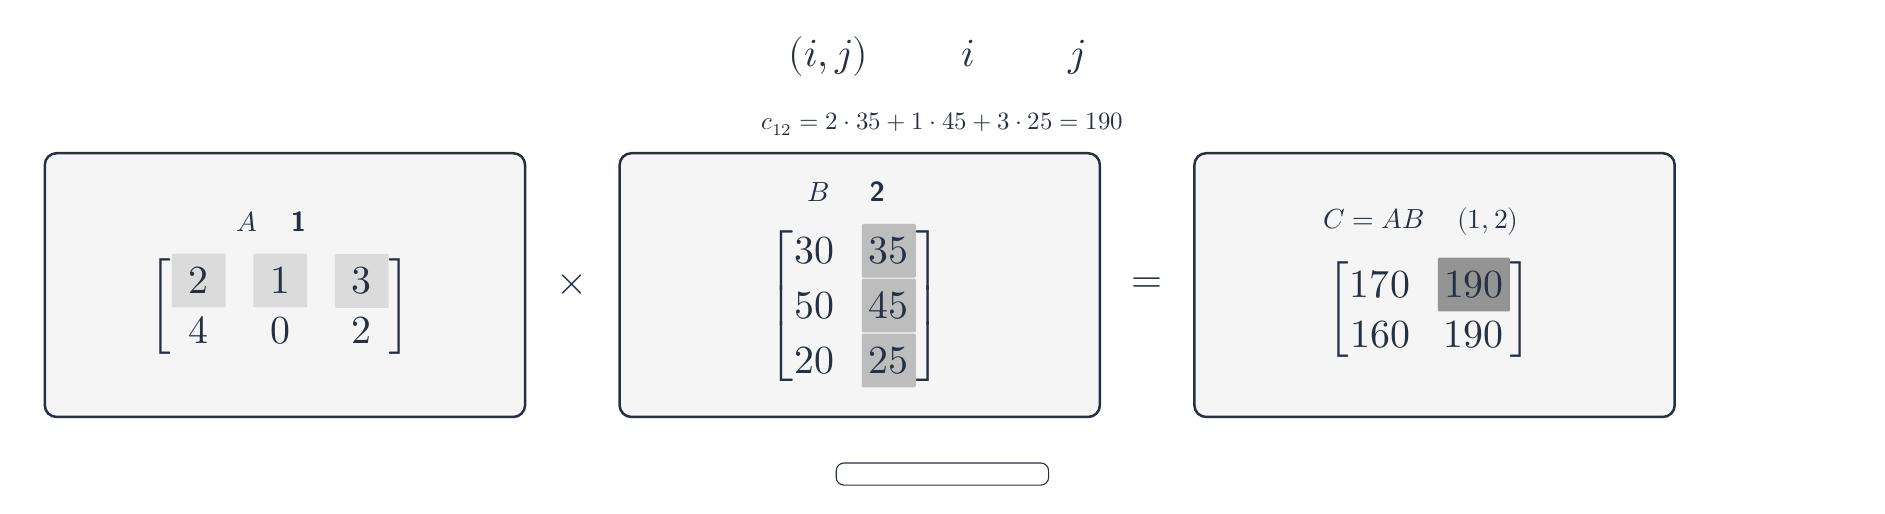
\begin{tikzpicture}[figure]
  \node[font=\bfseries\Large,align=center,text width=23cm] at (11.5,5.85)
    {乘積的第 $(i,j)$ 元由左矩陣第 $i$ 列與右矩陣第 $j$ 行配對加總};
  \node[font=\small] at (11.5,5.0)
    {$c_{12}=2\cdot35+1\cdot45+3\cdot25=190$};

  \node[panel,minimum width=6.1cm,minimum height=3.35cm] (A) at (3.15,2.95) {%
    \begin{minipage}{5.5cm}\centering
      \textbf{$A$：取第 1 列}\\[7pt]
      \Large$\begin{bmatrix}
        \RowCell{2}&\RowCell{1}&\RowCell{3}\\
        4&0&2
      \end{bmatrix}$
    \end{minipage}
  };
  \node[font=\Large] at (6.8,2.95) {$\times$};
  \node[panel,minimum width=6.1cm,minimum height=3.35cm] (B) at (10.45,2.95) {%
    \begin{minipage}{5.5cm}\centering
      \textbf{$B$：配對第 2 行}\\[7pt]
      \Large$\begin{bmatrix}
        30&\ColumnCell{35}\\
        50&\ColumnCell{45}\\
        20&\ColumnCell{25}
      \end{bmatrix}$
    \end{minipage}
  };
  \node[font=\Large] at (14.1,2.95) {$=$};
  \node[panel,minimum width=6.1cm,minimum height=3.35cm] (C) at (17.75,2.95) {%
    \begin{minipage}{5.5cm}\centering
      \textbf{$C=AB$：得到 $(1,2)$ 元}\\[7pt]
      \Large$\begin{bmatrix}
        170&\ResultCell{190}\\
        160&190
      \end{bmatrix}$
    \end{minipage}
  };

  \node[draw=FigureInk,rounded corners=1mm,fill=white,inner xsep=8pt,inner ysep=4pt,
        font=\scriptsize] at (11.5,0.55)
    {淺灰列與中灰行共享三個品項位置；深灰結果格保存三項乘積的總和。};
\end{tikzpicture}
\end{document}
